% Source: graduate-coursework/Sp26/CSCE775/course_notes/markov_reward_process.tex

\documentclass[border=4pt]{standalone}
\usepackage{amsmath, amssymb, amsthm}
\usepackage{graphicx}
\usepackage{tikz}
\usetikzlibrary{arrows.meta, positioning, automata, calc, decorations.markings}

\definecolor{garnet}{HTML}{73000A}

\begin{document}
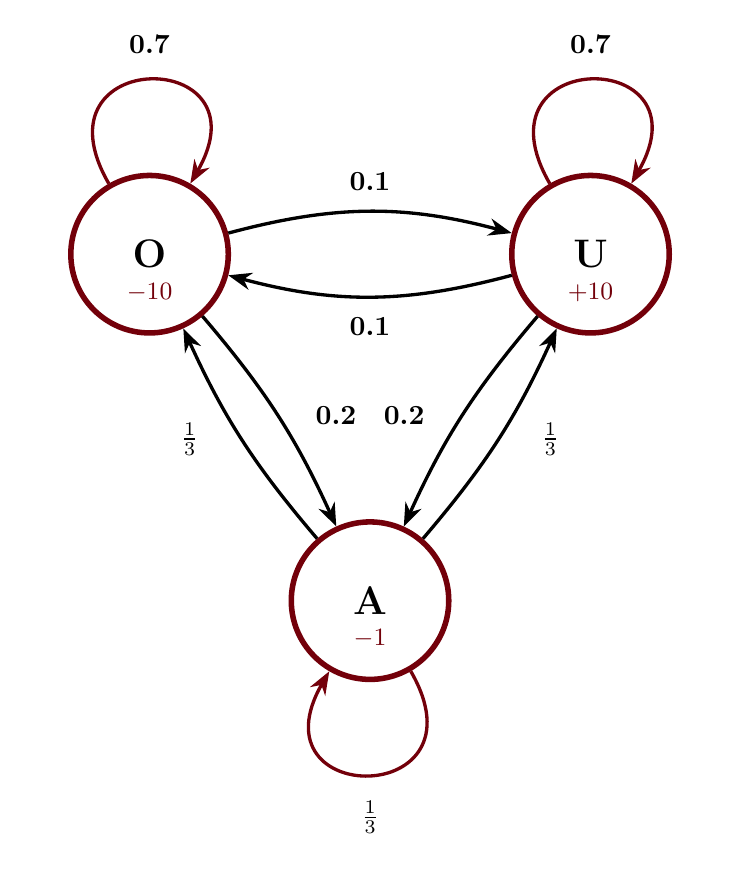
\begin{tikzpicture}[
    >=Stealth,
    scale=0.8,
    every state/.style={
        fill=white,
        draw=garnet,
        line width=2pt,
        text=black,
        minimum size=2cm,
        font=\bfseries\Large
    },
    every edge/.style={
        draw=black,
        line width=1.2pt,
        ->,
        >=Stealth
    },
    prob/.style={
        font=\bfseries,
        text=black,
        fill=white,
        inner sep=3pt
    },
    statelabel/.style={
        font=\small\bfseries,
        text=garnet
    }
]

% States
\node[state] (O) at (0, 0) {O};
\node[statelabel, below=1pt of O.center, yshift=-6pt] {$-10$};

\node[state] (U) at (7, 0) {U};
\node[statelabel, below=1pt of U.center, yshift=-6pt] {$+10$};

\node[state] (A) at (3.5, -5.5) {A};
\node[statelabel, below=1pt of A.center, yshift=-6pt] {$-1$};

% Self-loops
\path (O) edge[loop above, looseness=5, out=120, in=60, draw=garnet] node[prob, above=6pt] {0.7} (O);
\path (U) edge[loop above, looseness=5, out=120, in=60, draw=garnet] node[prob, above=6pt] {0.7} (U);
\path (A) edge[loop below, looseness=5, out=-60, in=-120, draw=garnet] node[prob, below=6pt] {$\frac{1}{3}$} (A);

% O <-> U transitions
\path (O) edge[bend left=15] node[prob, above=4pt] {0.1} (U);
\path (U) edge[bend left=15] node[prob, below=4pt] {0.1} (O);

% O <-> A transitions
\path (O) edge[bend left=8] node[prob, right=10pt, pos=0.5] {0.2} (A);
\path (A) edge[bend left=8] node[prob, left=12pt, pos=0.5] {$\frac{1}{3}$} (O);

% U <-> A transitions
\path (U) edge[bend right=8] node[prob, left=10pt, pos=0.5] {0.2} (A);
\path (A) edge[bend right=8] node[prob, right=12pt, pos=0.5] {$\frac{1}{3}$} (U);

\end{tikzpicture}
\end{document}
